\documentclass{../../physics_notes}

\title{Quantum Mechanics 2}
\author{St Aidan's Physics Society}
\date{\today}

\usepackage{physics}

\begin{document}

\maketitle
\begin{figure*}[h!]
	\centering
	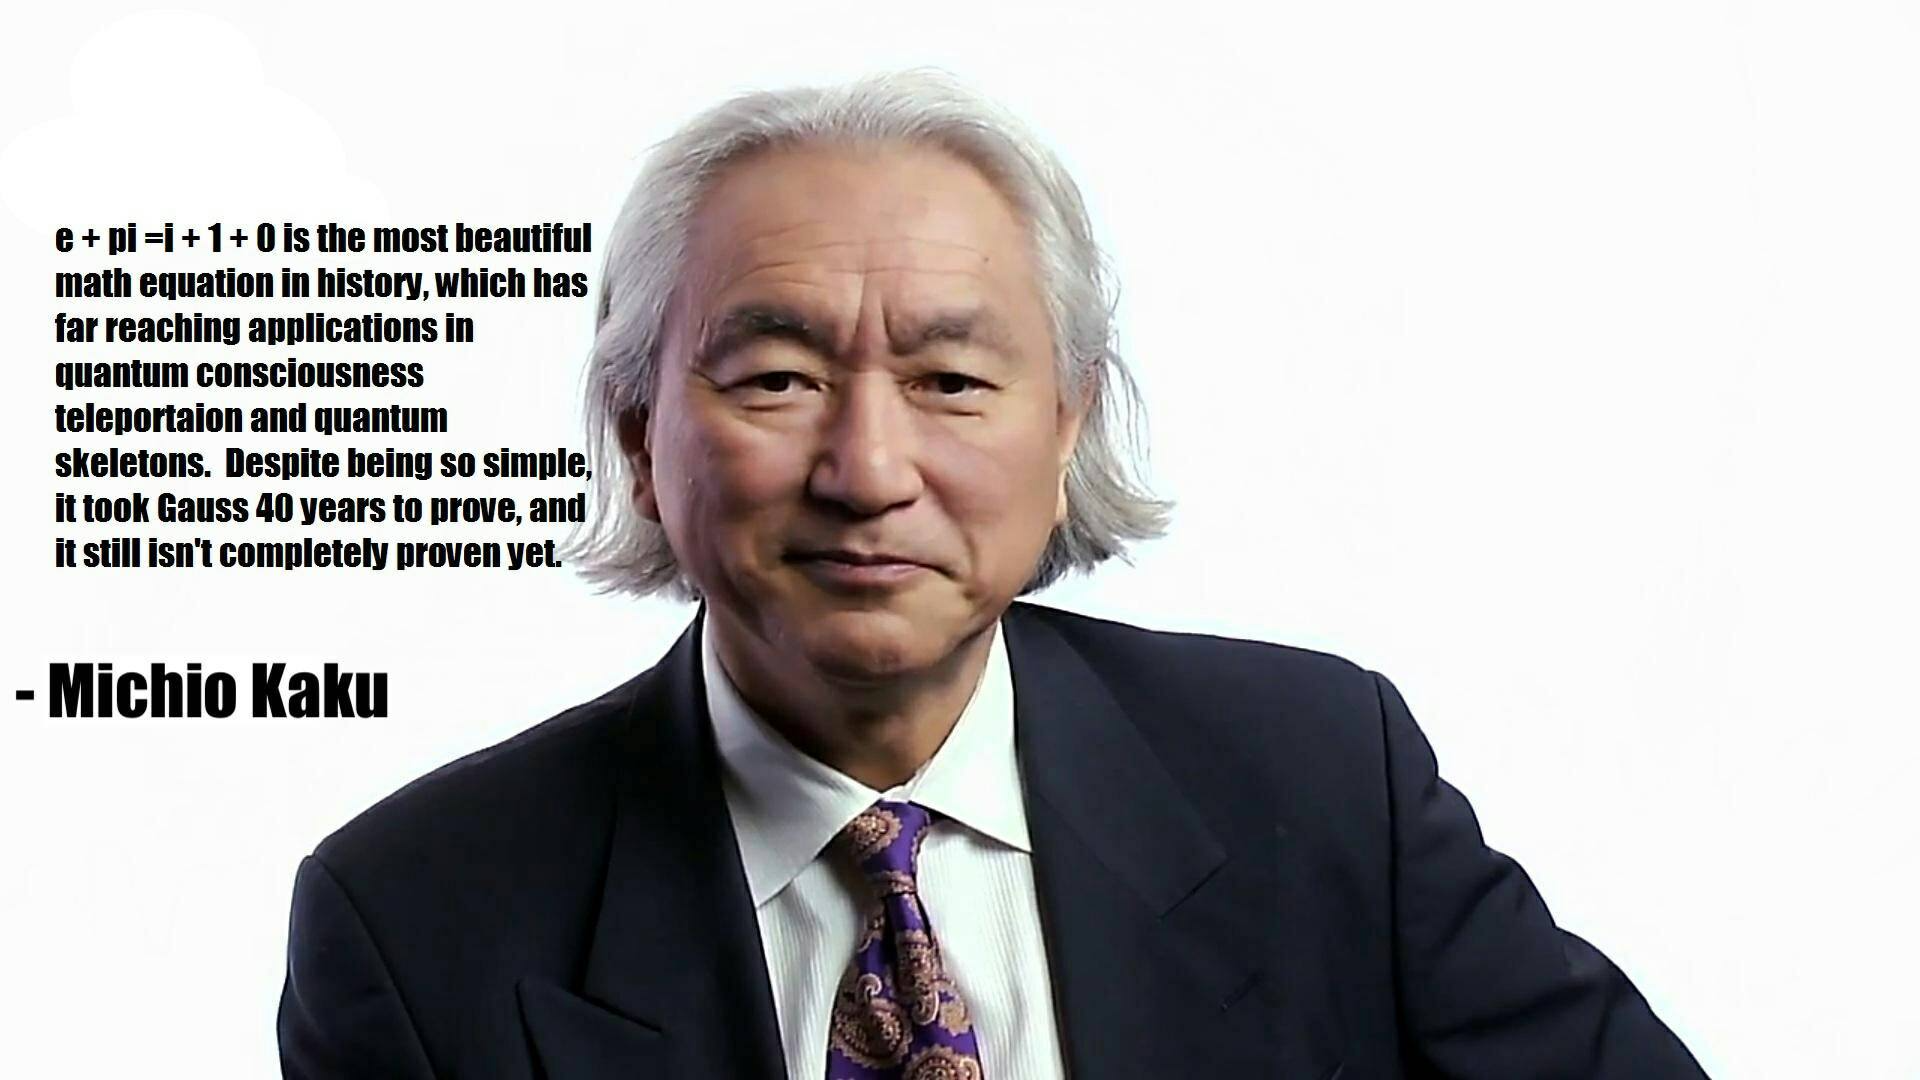
\includegraphics[width=\linewidth]{Figures/mich.png}
\end{figure*}
\tableofcontents
\newpage

\section*{Introduction}

These notes are designed to summarise the Foundations of Physics 2A (PHYS2581) Quantum Mechanics course, as taught by Prof. S Cole in the 2018/19 academic year. 

\section*{Summary}

\subsection*{The Five Postulates of Quantum Mechanics}

The content in this course can be summarised with the following five postulates:

\begin{enumerate}
	\item All possible predictions of the physical properties of a dynamical system can be obtained via its wavefunction.
	\item Every dynamical variable can be represented by a Hermitian operator, whose eigenvalues give the possible values of measurement of the dynamical variable. 
	\item The operators representing position and momentum are $x$ and $-i\hbar\nabla$ respectively. Operators for other dymanical variables can be derived using their corresponding dynaimcal variables' classical relations to position and momentum. 
	\item The probability of measuring a particular result of a superposition of states is given by the probability amplitude of the relevant eigenfunction, squared. 
	\item The time evolution of the wavefunction is described by the time-dependent Schr\"odinger equation.
\end{enumerate}

\section{Operators}\label{sec:operators}

All physical quantities in Quantum Mechanics can be represented by operators, which are essentially functions mapping from one space of physical states to another. From the $\hat{x} = x$ and $\hat{p} = -i\hbar\frac{\partial}{\partial x}$ operators along with time $t$, all other operators can be derived. For example, $\hat{E_k} = \frac{\hat{p}^2}{2m}$, as $E_k = \frac{p^2}{2m}$ classically. 

In quantum mechanics, these operators are made to act on wavefunctions (see §\ref{sec:wave_functions}): complex functions that describe everything we know about a system. The measureable values of the quantity represented by the general operator $\hat{Q}$ are the eigenvalues $q$ in the following eigenvalue problem:

\[ \hat{Q}\Psi = q\Psi \]

where $\Psi$ is the wavefunction of the system being measured. 

Classically, the Hamiltonian is usually the sum of kinetic and potential energies of a system. As such, we can define the Hamiltonian operator:

\begin{align*} 
\hat{H} &= \frac{\hat{p}^2}{2m} + V  \\
&= -\frac{\hbar^2}{2m} \frac{\partial^2}{\partial x^2} + V
\end{align*}

Using $\hat{H}{\Psi} = E\Psi$ (that the eigenvalues of the Hamiltonian are the allowed energy levels of the system), we obtain the Schr\"odinger equation. 


\subsection{Expectation}

The expectation of a general operator $\hat{Q}$ in 3D is given by:

\[ \expval{\hat{Q}} = \int_{V} \Psi^*\hat{Q}\Psi dV \]

The volume element $dV$ varies depending on the coordinate system. The volume element in some common 3D coordinate systems are given below. 

\begin{table}[h!]
\centering
	\begin{tabular}{c|c|c}
	Coordinate system & Position vector & Volume element \\ \hline
	Cartesian & $x\hat{\imath} + y\hat{\jmath} + z\hat{k}$ & $dxdydz$ \\
	Spherical polar & $r\sin{\theta}\cos{\phi}\hat{\imath} + r\sin{\theta}\sin{\phi}\hat{\jmath} + r\cos{\theta}\hat{k}$ & $r^2\sin{\theta}drd\theta d\phi$ \\
	Cylindrical polar & $\rho\cos{\theta}\hat{\imath} + \rho\sin{\theta}\hat{\jmath} + z\hat{k}$ & $\rho d\rho d\theta dz$
	\end{tabular}
	\caption{Volume element in common coordinate systems}
\end{table}
\subsection{Hermitian Operators}

If an operator $Q$ is Hermitian, then $Q^* = Q$. All operators that represent a real, measurable quantity are Hermitian as if $q$ is a measurable quantity, then we require that $q = q^*$, i.e. $q$ is real. So

\begin{align*}
\hat{Q}^*\Psi = q^*\Psi = q\Psi = \hat{Q}\Psi
\end{align*}

So $\hat{Q}^* = \hat{Q}$. Hence we see that if $q$ is measurable (and thus real), $\hat{Q}$ is Hermitian.


\subsection{Commutators}

The commutator of two operators $\hat{A}$, $\hat{B}$ is defined as $[\hat{A},\hat{B}] = \hat{A}\hat{B} - \hat{B}\hat{A}$. It follows that $[\hat{A},\hat{B}] = -[\hat{B},\hat{A}]$. If $[\hat{A},\hat{B}] =[\hat{B},\hat{A}] = 0$, then $\hat{A}$ and $\hat{B}$ are said to commute, meaning they share a common set of eigenfunctions.  Some important commutator identities are given below:

\begin{itemize}
	\item $[\hat{A},\hat{A}] = 0$
	\item $[\hat{A} + \hat{B}, \hat{C}] = [\hat{A},\hat{C}] + [\hat{B},\hat{C}]$
	\item $[\hat{A}\hat{B},\hat{C}] = \hat{A}[\hat{B},\hat{C}] + [\hat{A},\hat{C}]\hat{B}$
	\item $[\hat{A},\hat{B}\hat{C}] = [\hat{A},\hat{B}]\hat{C} + \hat{B}[\hat{A},\hat{C}]$
\end{itemize}

\subsection{Angular Momentum operators}

Two forms of angular momentum are important in quantum mechancics: orbital, and rotational. We will consider these separately, before looking at a more generalised approach.

\subsubsection*{Orbital Angular Momentum}

Orbital angular momentum is key for describing central potentials in 3D (e.g. the Hydrogen atom). Classically, orbital angular momentum, $\vec{L}$, is given by:

\begin{align*} \vec{L} = \vec{r} \times \vec{p} &= \begin{vmatrix} \hat{\imath} & \hat{\jmath} & \hat{k} \\ x & y & z \\ p_x & p_y & p_z \end{vmatrix} \\ &= (yp_z - zp_y)\hat{\imath} + (zp_x - xp_z)\hat{\jmath} + (xp_y - yp_x)\hat{k} \\ &= L_x \hat{\imath} + L_y \hat{\jmath} + L_z \hat{k} \end{align*}

with $L_x = (yp_z - zp_y)$, $L_y = (zp_x - xp_z)$, and $L_z = (xp_y - yp_x)$. Replacing position and mometum with their corresponding operators gives:

\begin{align*}
\hat{L_x} &= -i\hbar\left(y\frac{\partial}{\partial z} - z\frac{\partial}{\partial y}\right) \\
\hat{L_y} &= -i\hbar\left(z\frac{\partial}{\partial x} - x\frac{\partial}{\partial z}\right) \\
\hat{L_z} &= -i\hbar\left(x\frac{\partial}{\partial y} - y\frac{\partial}{\partial x}\right) 
\end{align*}

All three of these operators are Hermitian, and they do not commute with eachother. In fact, $[\hat{L_x}, \hat{L_y}] = i\hbar\hat{L_z}$, $[\hat{L_y}, \hat{L_z}] = i\hbar\hat{L_x}$, $[\hat{L_z}, \hat{L_x}] = i\hbar\hat{L_y}$. This non-commutation means we can only know the component of orbital angular momentum in one direction at any time, and gives rise to an uncertainty principle:

\[ \sigma_{\hat{L_x}}\sigma_{\hat{L_y}} \geq \frac{1}{2}\left|\expval{[\hat{L_x},\hat{L_y}]}\right| = \frac{\hbar}{2}\left|\expval{\hat{L_z}}\right| \]

However, we can obtain more information about the system by defining $\hat{L^2} = \hat{L_x^2} + \hat{L_y^2} + \hat{L_z^2}$ as we see $[\hat{L^2},\hat{L_x}] = [\hat{L^2}, \hat{L_y}] = [\hat{L^2}, \hat{L_z}] = 0$, and so we can know a component of orbital angular momentum and the total angular momentum simultaneously. 
\subsection{Ladder Operators}

\section{Foundations of Quantum Mechanics}\label{sec:foundations}
\subsection{The Quantum Wavefunction}

A consequence of wave-particle duality is that what would classically be considered as discrete particles, such as electrons, can be described via a wavefunction (analagous to a classical wave equation). In order for an arbitrary wavefunction $\Psi(\vec{r}, t)$ to be valid, it has to obey the Schr\"odinger equation (given here in its 3D time-dependent form):

\[ \hat{H}\Psi = i\hbar\frac{\partial\Psi}{\partial t} \]

where $\hat{H} = -\frac{\hbar^2}{2m}\nabla^2 + V(\vec{r}, t)$ is the Hamiltonian operator defined previously. A useful alternate form of the equation is the 1D time-independent Schr\"odinger equation:

\[ \hat{H}\Psi = E\Psi \]

where $E$ is the total energy of the system, and the Hamiltonian in 1D is $\hat{H} = -\frac{\hbar^2}{2m}\frac{\partial^2}{\partial x^2} + V(x)$.

\subsubsection{Probability distributions and normalisation}

A further requirement for a wavefuntion to be valid in real space is for the total probability of finding the particle at some position in space is equal to 1. The probability of finding a particle described by the complex unnormalised wavefunction $f(x,t)$ between $x$ and $x+dx$ is:

\[ P(x,t)dx \propto \left|f(x,t)\right|^2 dx = f^*(x,t)f(x,t) dx \]

where the constant of proportionality is the normalisation constant $N$, given by:

\[ N = \frac{1}{\sqrt{\int_{-\infty}^{+\infty} \left|f(x,t)\right|^2 dx}} \]

So $\Psi(x,t) = Nf(x,t)$ and $\int_{-\infty}^{+\infty} P(x,t)dx = \int_{-\infty}^{+\infty} \Psi^*(x,t)\Psi(x,t)dx = 1$.

\subsubsection{Dirac notation}

In Dirac notation, devised by Paul Dirac, bra and ket vectors are used to represent wave functions and their complex conjugates:

\begin{align*} 
\text{(ket):\;} &\ket{\psi} = \psi; \\ 
\text{(bra):\;} &\bra{\psi} = \psi^*; 
\end{align*}

They can be used together to represent the expectation of an operator $\hat{Q}$:

\[ \expval{\hat{Q}} = \expval{\hat{Q}}{\psi} = \int_{V} \psi^*\hat{Q}\psi dV \]

This alternative notation provides a very elegant way of dealing with the maths of Quantum Mechanics. 

\subsection{Eigenfunctions of the Schr\"odinger equation}

We have seen the time-independent Schr\"odinger equation expressed in the form of an eigenvalue problem:

\[ \hat{H}\psi_E(x) = E\psi_E(x) \]

Where $E$ is the eigenvalue corresponding the eigenfunction (often referred to as an eigenstate) $\psi_E(x)$. What we have previously referred to as the wavefunction $\Psi$ is actually the weighted sum of the eigenstates of the system with the time-dependece included, over all of the possible energy levels:

\[ \Psi(x,t) = \sum_E c_E \psi_E(x,t) e^{-\frac{iEt}{\hbar}} \]

This time-dependence of energy can be derived from the fact that the time-dependent Schr\"odinger equation is separable into two ODEs, giving the solution $\Psi_E(x,t) = X_E(x)T_E(t) = \psi_E(x)e^{-\frac{iEt}{\hbar}}$. Note that the total wavefunction given above is \emph{not} a solution of the time-independent Schr\"odinger equation. 

A useful property is that eigenfunctions corresponding to different eigenvalues are orthogonal, meaning that for normalised eigenfunctions $\psi_n$ and $\psi_m$ given by

\begin{align*}
\hat{H}\psi_n &= E_n\psi_n \\
\hat{H}\psi_m &= E_m\psi_m
\end{align*}

we have that $\int \psi_n \psi_m^* = \delta_{nm}$ where $\delta$ is the Kronecker delta. 

The eigenfunctions of an operator form a complete basis of the space containing every possible state of the system - this is explored in greater depth in the PHYS2631 Quantum Theory course. A system can exist in a superposition of several eigenstates, where each state has a probability of being measured. The act of measurement is said to `collapse' the wavefunction to the eigenstate corresponding to the measured value of the physical quantity in question, by making the probability of being found in all other eigenstates zero. 

We see that if $\psi(x) = \sum_E c_E \psi_E(x) $, then 

\[ \expval{E} = \sum_m |c_m|^2E_m \]

It turns out that $|c_m|^2$ is the probability of measuring the superposition of states to be in the state $\psi_m$ with energy $E_m$. We can calculate these $c_m$ using the following relation (a justification for this is given in the course notes, §6.2):

\[ c_m = \int\psi^*_m\psi dx = \bra{\psi_m}\ket{\psi}\]

Including the time-dependence of each state leads us to find that superpositions of eigenfunctions are not stationary states (that is, they vary with time) unlike eigenstates, which have no time-dependence. 

\subsection{Angular Momentum Operators}

Classically, objects can have two forms of angular momentum: orbital, and rotational. We can reformulate orbital angular momentum using operators without straying too far from the classical interpretation, however rotational angular momentum is only present in Quantum Mechanics as an analogy. The nature of electrons as pointlike particles means that any notion of them rotating is meaningless, nevertheless experiment has shown that fundamental particles posess an intrinsic, quantised angular momentum which we call `spin'. Once we have looked at both forms, we can generalise the concept of angular momentum.

\subsubsection{Orbital angular momentum}

Orbital angular momentum is key for describing central potentials in 3D (e.g. the Hydrogen atom). Classically, orbital angular momentum, $\vec{L}$, is given by:

\begin{align*} \vec{L} = \vec{r} \times \vec{p} &= \begin{vmatrix} \hat{\imath} & \hat{\jmath} & \hat{k} \\ x & y & z \\ p_x & p_y & p_z \end{vmatrix} \\ &= (yp_z - zp_y)\hat{\imath} + (zp_x - xp_z)\hat{\jmath} + (xp_y - yp_x)\hat{k} \\ &= L_x \hat{\imath} + L_y \hat{\jmath} + L_z \hat{k} 
\end{align*}

with $L_x = (yp_z - zp_y)$, $L_y = (zp_x - xp_z)$, and $L_z = (xp_y - yp_x)$. Replacing position and mometum with their corresponding operators gives:

\begin{align*}
\hat{L_x} &= -i\hbar\left(y\frac{\partial}{\partial z} - z\frac{\partial}{\partial y}\right) \\
\hat{L_y} &= -i\hbar\left(z\frac{\partial}{\partial x} - x\frac{\partial}{\partial z}\right) \\
\hat{L_z} &= -i\hbar\left(x\frac{\partial}{\partial y} - y\frac{\partial}{\partial x}\right) 
\end{align*}

All three of these operators are Hermitian, and they do not commute with each other. In fact, $[\hat{L_x}, \hat{L_y}] = i\hbar\hat{L_z}$, $[\hat{L_y}, \hat{L_z}] = i\hbar\hat{L_x}$, $[\hat{L_z}, \hat{L_x}] = i\hbar\hat{L_y}$. This non-commutation means we can only know the component of orbital angular momentum in one direction at any time, and gives rise to an uncertainty principle:

\[ \sigma_{\hat{L_x}}\sigma_{\hat{L_y}} \geq \frac{1}{2}\left|\expval{[\hat{L_x},\hat{L_y}]}\right| = \frac{\hbar}{2}\left|\expval{\hat{L_z}}\right| \]

However, we can obtain more information about the system by defining the total angular momentum $\hat{L^2} = \hat{L_x^2} + \hat{L_y^2} + \hat{L_z^2}$ as we see $[\hat{L^2},\hat{L_x}] = [\hat{L^2}, \hat{L_y}] = [\hat{L^2}, \hat{L_z}] = 0$, and so we can know a component of orbital angular momentum and the total angular momentum simultaneously. 

The set of eigenfunctions common to $\hat{L_z}$ and $\hat{L^2}$, which we refer to as $Y_{lm}(\theta, \phi)$ are known as spherical harmonics and are defined such that:

\[ \hat{L_z}Y_{lm}(\theta, \phi) = m\hbar Y_{lm}(\theta, \phi) \]
\[ \hat{L^2}Y_{lm}(\theta, \phi) = l(l+1)\hbar^2 Y_{lm}(\theta, \phi) \]

where $l$ and $m$ are integers with $|m| \leq l$, meaning for each value of $l$ there are $2l+1$ possible values for $m$. The exact form of these spherical harmonics is given in the course notes, §10.4, however the following general form is useful to know:

\[ Y_{lm}(\theta, \phi) = \Theta_{lm}(\theta)\Phi_m(\phi) = \Theta_{lm}(\theta)e^{im\phi} \]

This means that we can extract a probability distribution in $\theta$ by integrating over $\phi$:

\begin{align*} 
P(\theta)d\theta = \int_{\phi=0}^{\phi=2\pi} P(\theta, \phi) d\Omega &= \int_{\phi=0}^{\phi=2\pi} Y^*_{lm}(\theta, \phi) Y_{lm}(\theta, \phi) \sin{\theta} d\theta d\phi \\
&= \int_{\phi=0}^{\phi=2\pi} \Theta_{lm}^* \Theta_{lm} \sin{\theta} d\theta d\phi \\
&= 2\pi \left| \Theta_{lm}(\theta)\right|^2 \sin{\theta} d\theta
\end{align*}

where $P(\theta, \phi) d\Omega$ is the probability of finding the particle in some solid angle $d\Omega = \sin{\theta} d\theta d\phi$ around $(\theta, \phi)$.

\subsubsection{Spin}

The Stern-Gerlach experiment provided evidence for intrinsic angular momentum of electrons, and showed that this `spin' can take two values (see course notes, §13.1 for more). As with all quantites in Quantum Mechanics, we can represent spin with an operator $\hat{S_z}$, which has the following eigenstates in the case of an electron:

\begin{align*}
\hat{S_z}\ket{\chi_+} &= \frac{\hbar}{2}\ket{\chi_+} \\
\hat{S_z}\ket{\chi_-} &=  -\frac{\hbar}{2}\ket{\chi_-}
\end{align*}

We refer to $\ket{\chi_+}$ as spin-up and $\ket{\chi_-}$ as spin-down.

\subsubsection*{Magnetic moment}

By considering the definition of the magnetic moment $\mu = IA$ we can derive a magnetic moment due to the orbital motion of an electron:

\[ \vec{\hat{\mu_l}} = -\frac{\mu_B}{\hbar} \vec{\hat{L}} \]

where $\mu_B = \frac{e\hbar}{2m_e}$ is the Bohr magneton. The $z$-component of this moment is given by:

\[ (\hat{\mu_l})_z = -\frac{\mu_B}{\hbar} \hat{L_z} \]

There is also a magnetic moment associated with spin, given by:

\[ \vec{\hat{\mu_s}} = -g_s \frac{\mu_B}{\hbar} \vec{\hat{S}} \]

where $g_s$ is the spin g-factor. Hence the $z$-component of spin magnetic moment is:

\[ (\hat{\mu_s})_z = -g_s m_s \mu_B  \approx \mp \mu_B \]

where $m_s = \pm\frac{1}{2}$ is the quantum number corresponding to the spin states $\ket{\chi_+}$ and $\ket{\chi_-}$.

\subsubsection{Ladder operators}

In the case of orbital angular mometum $\vec{\hat{L}}$, we can define ladder operators $\hat{L_\pm} = \hat{L_x} \pm i\hat{L_y}$, with:

\begin{align*} 
[\hat{L^2}, \hat{L_\pm}] &= [\hat{L^2}, \hat{L_x}] \pm i[\hat{L^2}, \hat{L_y}] \\
&= 0 \pm i (0) \\
&= 0 
\end{align*}

Hence we can show:

\[ \hat{L^2}(\hat{L_\pm}f_{\lambda, \mu}) = \lambda \hbar^2 \hat{L_\pm} f_{\lambda, \mu} \]

Note that this does not imply that $\hat{L^2}$ and $\hat{L_\pm}$ have a common set of eigenstates, as $\hat{L_\pm}$ does not correspond to a physical observable as it is not Hermitian. 

We also have:

\begin{align*}
[\hat{L_z}, \hat{L_\pm}] &= [\hat{L_z}, \hat{L_x}] \pm i[\hat{L_z}, \hat{L_y}] \\
&= i\hbar\hat{L_y} \pm i(-i\hbar\hat{L_x}) \\
&= i\hbar\hat{L_y} \pm \hbar\hat{L_x} \\
&= \hbar (\pm\hat{L_x} + i\hat{L_y}) \\
&= \pm\hbar(\hat{L_x} \pm i\hat{L_y}) \\
&= \pm\hbar\hat{L_\pm}
\end{align*}

This allows us to show:

\[ \hat{L_z}(\hat{L_\pm}f_{\lambda, \mu}) = (\mu \pm 1)\hbar \hat{L_\pm} f_{\lambda, \mu} \]

So we see that ladder operators $\hat{L_\pm}$ increase and decrease the quantum number $\mu$ by $1$ respectively: ascending and descending the `ladder' of possible values.

We have seen previously that $-\lambda \leq \mu \leq \lambda$, meaning there must be a top and bottom rung to the ladder, where $\hat{L_+}f_{\lambda, \mu_\text{max}} = 0$ and $\hat{L_-}f_{\lambda, \mu_\text{min}} = 0$. This leads us to find that $\lambda = \mu_\text{max}(\mu_\text{max} + 1) = \mu_\text{min}(\mu_\text{min} - 1)$ which implies $\mu_\text{min} = -\mu_\text{max}$, and that $\mu_\text{max} = \frac{N}{2}$ where $N$ is the number of rungs on the ladder. Hence we see that $\mu$ can take integer values between $-\lambda$ and $\lambda$.

\subsubsection{Generalised angular momentum}

We have seen that, in general, angular momentum operators obey a set of conditions. We can define a general angular momentum $\vec{\hat{J}}$ with total general angular momentum $\hat{J^2}$, where:

\begin{itemize}
	\item $\hat{J^2}$ and $\hat{J_z}$ have a common set of eigenfunctions $f_{j,m_j}$, with \[ \hat{J^2}f_{j,m_j} = j(j+1)\hbar^2 f_{j,m_j} \] \[ \hat{J_z}f_{j,m_j} = m_j\hbar f_{j,m_j} \]
	\item A pair of ladder operators $\hat{J_\pm} = \hat{J_x} \pm i\hat{J_y}$ exist, with \[ \hat{J_z}\hat{J_+}f_{j,m_j} = (m_j + 1)\hbar \hat{J_+} f_{j,m_j} \] \[ \hat{J_z}\hat{J_-}f_{j,m_j} = (m_j - 1)\hbar \hat{J_-} f_{j,m_j} \] In other words, $\hat{J_+}$ raises $m_j$ by one, and $\hat{J_-}$ reduces $m_j$ by one.
	\item $j$ can take integer \emph{or} half-integer values: $j = 0, 1, 2, ...$ or $j = \frac{1}{2}, \frac{3}{2}, \frac{5}{2}, ...$
	\item $m_j$ runs in integer steps from $-j$ to $j$
\end{itemize}

We can deduce these last two points from the ladder operators (see course notes, §§12.3-12.5).

\subsection{Theorems and Principles}
\subsubsection{The uncertainty principle}

The general uncertainty principle for two non-commutating operators is given by: (derivation in Appendix B of course notes)

\[ \sigma_{A}^2 \sigma_{B}^2 \geq \left(\frac{1}{2i} \expval{[\hat{A}, \hat{B}]} \right)^2 = \left(\frac{1}{2i} \expval{\hat{A}\hat{B}} - \expval{\hat{B}\hat{A}} \right)^2\]

In the case of $\hat{x}$ and $\hat{p}$, we know $\expval{[\hat{A}, \hat{B}]} = [\hat{A}, \hat{B}] = i\hbar$ so the above inequality leads to the well-known position-momentum uncertainty principle:

\[ \sigma_x \sigma_p = \Delta x \Delta p \geq \frac{\hbar}{2} \]

\subsubsection{Time evolution of expectation values}

In general, taking the time derivative of an expectation value gives 

\[ \frac{d\expval{\hat{Q}}}{dt} = \frac{d}{dt}\bra{\psi}\hat{Q}\ket{\psi} = \left(\frac{\partial\bra{\psi}}{\partial t}\right) \hat{Q}\ket{\psi} + \bra{\psi}\frac{\partial \hat{Q}}{\partial t}\ket{\psi} + \bra{\psi}\hat{Q}\left(\frac{\partial \ket{\psi}}{\partial t}\right) \]

From the Schr\"odinger equation, we find

\[ \frac{\partial\ket{\psi}}{\partial t} = -\frac{i\hat{H}}{\hbar}\ket{\psi} \]

where $\hat{H}$ is the Hamiltonian. Taking the complex conjugate of both sides gives:

\[ \frac{\partial \bra{\psi}}{\partial t} = \bra{\psi}\frac{i\hat{H}}{\hbar} \]

Hence we find 

\[ \frac{d \expval{\hat{Q}}}{d t} = \frac{i}{\hbar}\expval{[\hat{H}, \hat{Q}]} + \expval{\frac{\partial \hat{Q}}{\partial t}} \]

\subsubsection{Ehrenfest theorems}

Using the previous result for the time-dependence of the expectation of an operator to the position operator, with $\hat{H} = \frac{\hat{p}^2}{2m} + V(x)$ gives

\[ \frac{d\expval{\hat{x}}}{dt} = \frac{i}{\hbar}\expval{[\hat{H}, \hat{x}]} + \expval{\frac{\partial \hat{x}}{\partial t}} \]

Given that the position operator itself is time-independent, this reduces to

\begin{align*} 
	\frac{d\expval{\hat{x}}}{dt} &= \frac{i}{\hbar}\expval{[\hat{H}, \hat{x}]} \\
	&= \frac{i}{\hbar}\expval{-i\hbar\frac{\hat{p}}{m}} = \frac{\expval{\hat{p}}}{m}
\end{align*}

This is the first Ehrenfest theorem. The second, given below, is derived similarly:

\[ \frac{d\expval{\hat{p}}}{dt} = -\expval{\frac{dV}{dx}} \]

\subsubsection{Virial theorem}

Considering $\hat{Q} = \hat{x}\hat{p}$ and applying the time evolution equation, we find:

\[ \frac{d\expval{\hat{x}\hat{p}}}{dt} = \expval{\frac{\hat{p}^2}{m} - \hat{x}\frac{dV}{dx}} \]

For a state in equilibrium, $\frac{d\expval{\hat{x}\hat{p}}}{dt} = 0$ so

\[ \expval{\frac{\hat{p}^2}{m}} = \expval{\hat{x}\frac{dV}{dx}} \]

Or similarly

\[ \expval{T} = \frac{1}{2}\expval{\hat{x}\frac{dV}{dx}} \]

\subsubsection{The correspondance principle}

The correspondance principle, as proposed by Niels Bohr in 1920, states that quantum mechanics will agree with classical mechanics in the limit of large quantum numbers (i.e. when dealing with large energies). 

\section{Applications of Quantum Mechanics}\label{sec:applications}
\subsection{Eigenfunctions of various potentials}

\subsubsection{The infinite square well}

The infinite square well is an ideal quantum potential given in one dimension by

\[ V(x) = \left\{\begin{matrix}
\infty & \text{if} & x < 0 \\
0 & \text{if} & 0\leq x \leq L \\
\infty & \text{if} & x > L 
\end{matrix}\right. \]

Hence the Schr\"odinger equation in an infinite potential well is:

\[ -\frac{\hbar^2}{2m}\frac{d^2 \psi}{dx^2} = E\psi \]

Solving this 2nd order ODE and applying the boundary condition $\psi(0) = 0$ gives:

\[ \psi(x) = A\sin(kx)\text{, where } k = \frac{\sqrt{2mE}}{\hbar} \]

Normalising and applying the boundary condition $\psi(L) = 0$ gives

\[ \psi_n (x) = \sqrt{\frac{2}{L}}\sin(\frac{n\pi x}{L}) \text{ with } E = \frac{n^2 \pi^2 \hbar^2}{2m L^2} \]

Adding the time dependence leads to the full energy eigenfunctions:

\[ \Psi_n (x,t) = \psi_n (x) e^{-\frac{iE_n t}{\hbar}} = \sqrt{\frac{2}{L}}\sin(\frac{n\pi x}{L}) e^{-\frac{iE_n t}{\hbar}} \]




\subsubsection{The linear harmonic oscillator}

\subsection{Finding the Hydrogen Wavefunction}

\subsubsection*{Hydrogen atom in a magnetic field}

\section{Relativistic corrections}\label{sec:relativistic_corrections}
\subsection{Non-degenerate perturbation theory}
\subsection{Degenerate perturbation theory}
\subsection{The Hydrogen atom}
\subsubsection{Degenerate perturbation theory in hydrogen}
\subsubsection{Hydrogen fine splitting}




\end{document}